%FOR PDFLATEX USE ONLY
\documentclass[a4paper,12pt]{article}

\usepackage{amssymb,amsmath} %math symbols

\usepackage[margin=2cm]{geometry} %paper geometry

\usepackage[utf8]{inputenc} %allows unicode (including russian) source file
\usepackage[russian]{babel} %docment in russian-style
\usepackage[utf8]{inputenc}
\usepackage[unicode]{hyperref} %links inside of the text
\usepackage[pdftex]{graphicx} %includegraphics pictures
\usepackage{cmlgc} %bold text

\usepackage{array} %arrays

\usepackage{wrapfig}
\usepackage{array}
\usepackage{lipsum}
\usepackage{esvect}
\usepackage{hyperref}
\usepackage{xcolor}
\definecolor{linkcolor}{HTML}{799B03} % цвет ссылок
\definecolor{urlcolor}{HTML}{799B03} % цвет гиперссылок
 
\hypersetup{pdfstartview=FitH,  linkcolor=linkcolor,urlcolor=urlcolor, colorlinks=true}
 
\usepackage{subfig}
\usepackage{calc}
\usepackage{pgfplots,tikz,circuitikz}
\usepackage{pgfplotstable}
\usepackage{tkz-euclide}

\usepackage{centernot}
\usepackage{cancel}

\documentclass{article}
\usepackage{amsmath}
\usepackage{mathtext}
\usepackage[T1,T2a]{fontenc}
\usepackage[utf8]{inputenc}
\usepackage[english, bulgarian, russian]{babel}
\usepackage{tikz}
\usepackage{pgfplots}
\usepackage[export]{adjustbox}
\usepackage[left=2cm,right=2cm,
    top=2cm,bottom=2cm,bindingoffset=0cm]{geometry}




\renewcommand{\thesection}{\alph{section}}

\begin{document}



\maketitle
\begin{center}
\LARGE{МОЛЕКУЛЯРНАЯ ДИНАМИКА}\\
    \Large{Задание 3}\\
    Стрижак Даниил
\end{center}
\tableofcontents
\newpage

\section*{Аннотация}\addcontentsline{toc}{section}{Аннотация}

В работе исследуются применимости разных критериев плавления вещества, такие как калориметрический критерий, пропадание дальнего порядка, критерий Линдеманна и другие. \\
Вся работа выполнена с помощью библитеки lammps и вспомогательных скриптов python3. 

\section{Плавление кристаллов}

Путем изохорического нагрева кристалла при двух различных плотностях ($\rho_1 = 1.0 $ и $\rho_2 = 2.0$) получим жидкость. Видео плавления кристалла при плотности $\rho_1$ можно посмотреть на \href{https://youtu.be/tzXEO91IEJA}{YOUTUBE}. Построим зависимость энергии от температуры. Можно заметить скачок энергии при определенной температуре, обозначает плавление. В первом случае: $\Delta E \approx 0.6 $ при $T \approx 1.73$. Во втором случае: $\Delta E \approx 4.75$ при $T \approx 11.30$. 

\begin{minipage}{0.47\textwidth}
    \begin{center}
        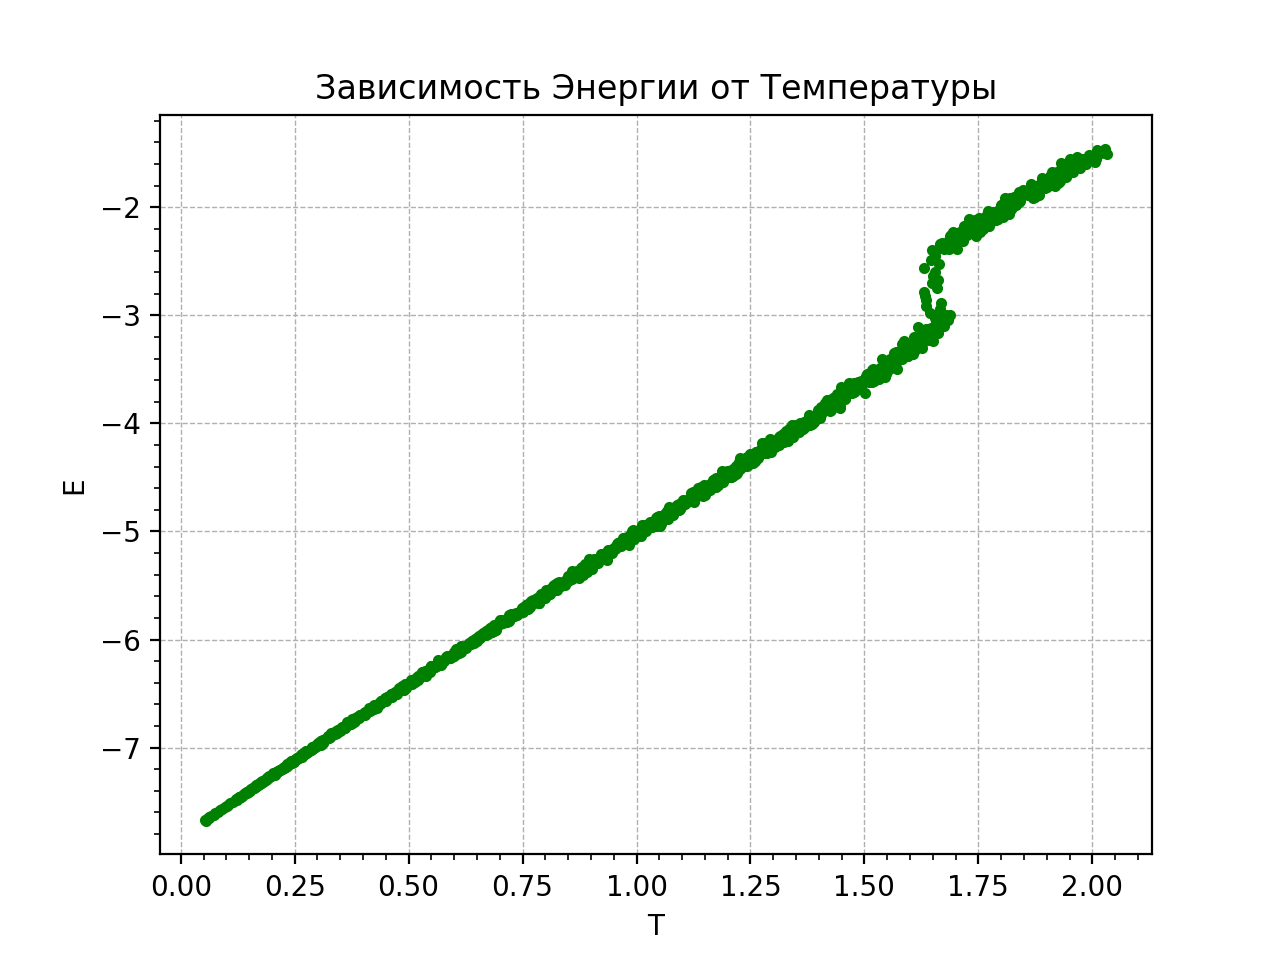
\includegraphics[width=0.9\linewidth]{1.png}\\
        Плотность -- $\rho_1 = 1.0$
    \end{center}
   
\end{minipage}
\begin{minipage}{0.47\textwidth}
    \begin{center}
        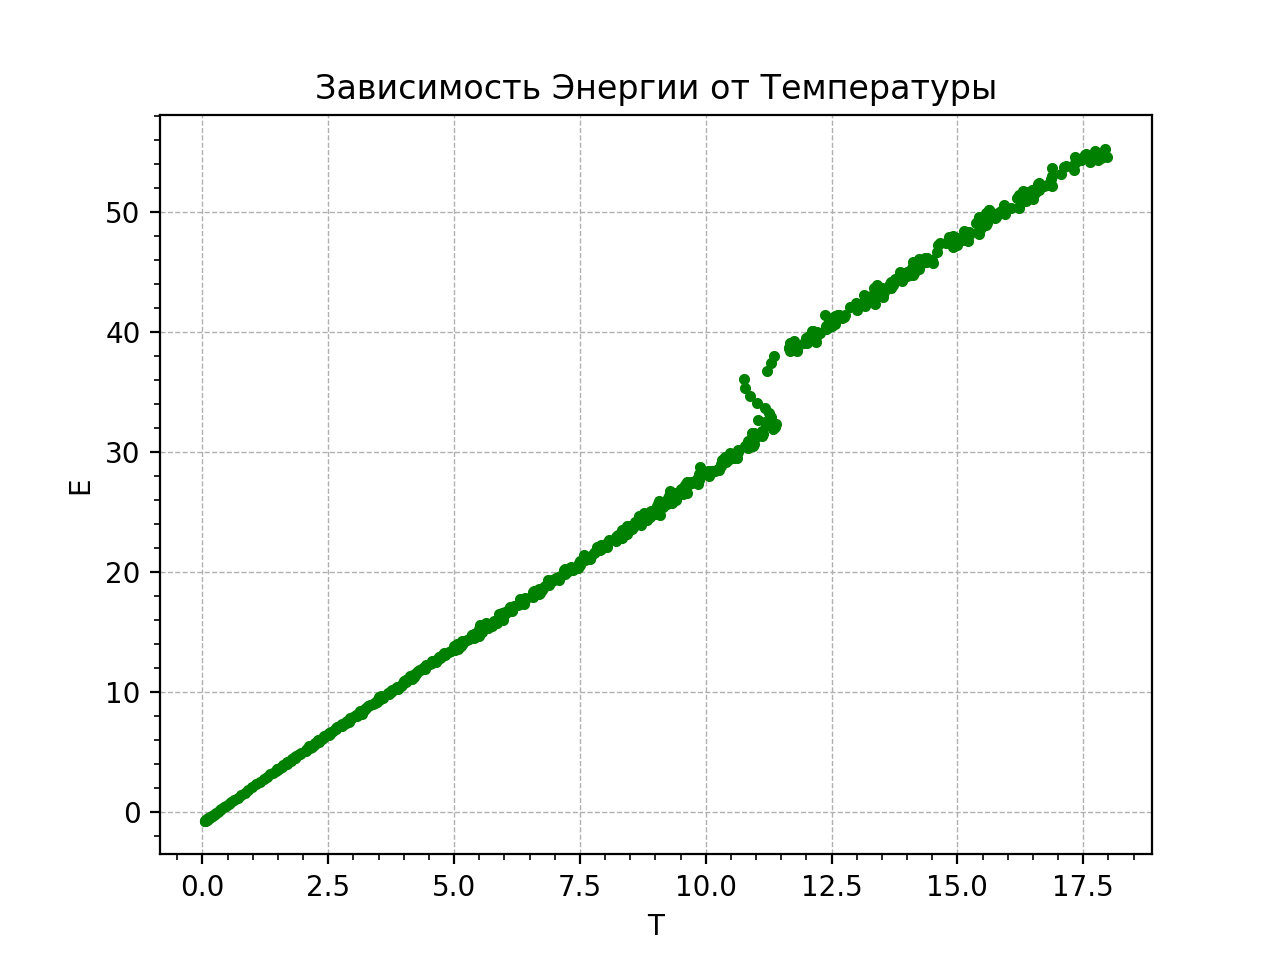
\includegraphics[width=0.9\linewidth]{2.png}\\
        Плотность -- $\rho_2 = 2.0$
    \end{center}
\end{minipage}

\section{Исчезновение дальнего порядка RDF}

Теперь рассмотрим радиальные функции распределения при различных температурах для плотности $\rho_1 = 1.0$. В самом начале радиальная функция распределения -- есть функция твердого тела, а в конце -- жидкости. 

\begin{minipage}{0.47\textwidth}
    \begin{center}
        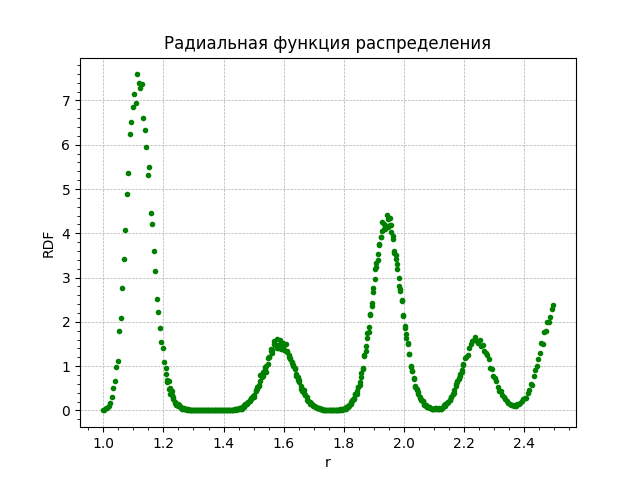
\includegraphics[width=0.9\linewidth]{3.png}\\
        Твердое тело
    \end{center}
   
\end{minipage}
\begin{minipage}{0.07\textwidth}
\begin{center}

\Longrightarrow

\end{center}
\end{minipage}
\begin{minipage}{0.47\textwidth}
    \begin{center}
        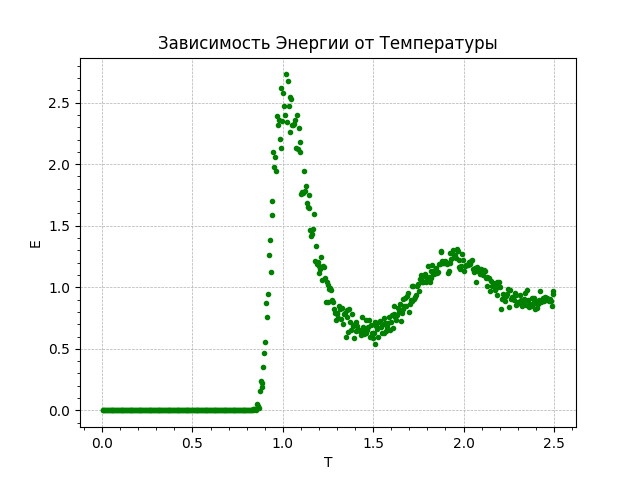
\includegraphics[width=0.9\linewidth]{4.png}\\
        Жидкость
    \end{center}
\end{minipage}

\newpage

Рассмотрим участок, выделенный на рисунке ниже и построим RDF для этого участка. Видно, что дальний порядок пропадает, тело переходит из одной фазы в другую. Однако дальний порядок пропадает несколько раньше, чем происходит скачок энергии (при температуре 1.52, в не предыдущей 1.73), что может говорить о неточности определения фазового перехода таким методом. 


\begin{center}
        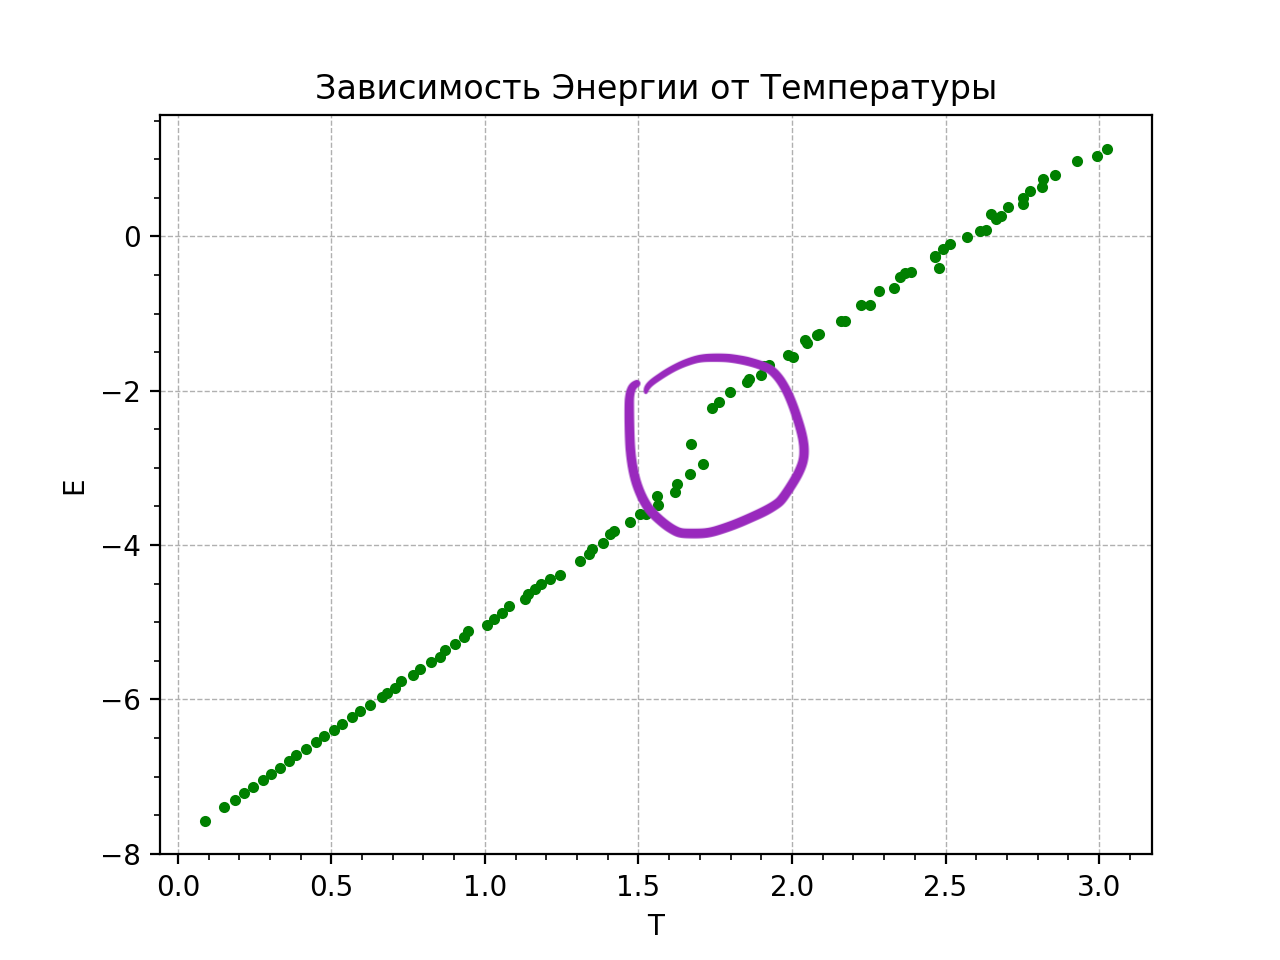
\includegraphics[width=0.5\linewidth]{5.png}\\
        \end{center}
\begin{center}
        Плотность $\rho_1 = 1.0$
\end{center}

\begin{minipage}{0.3\textwidth}
    \begin{center}
        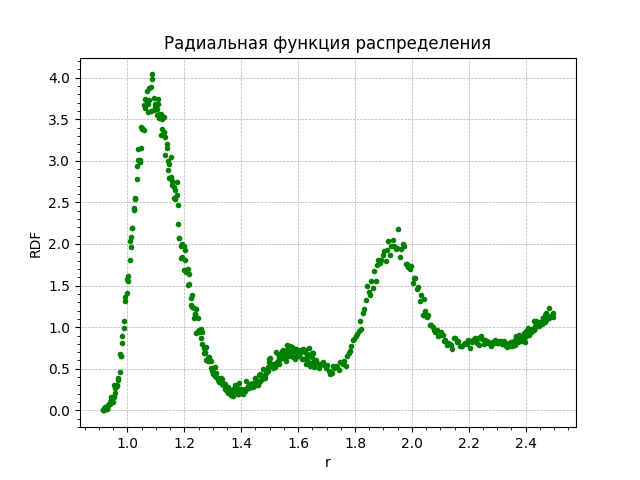
\includegraphics[width=\linewidth]{6.png}\\
        25000 шаг
    \end{center}
   
\end{minipage}
\begin{minipage}{0.05\textwidth}
\begin{center}

\Longrightarrow

\end{center}
\end{minipage}
\begin{minipage}{0.3\textwidth}
    \begin{center}
        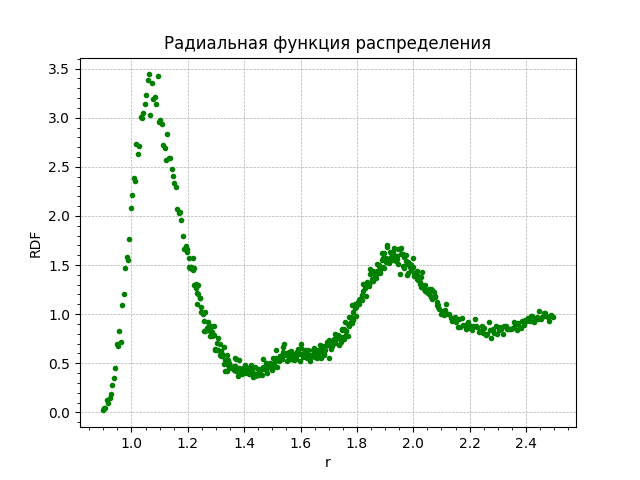
\includegraphics[width=\linewidth]{7.png}\\
        30000 шаг
    \end{center}
\end{minipage}
\begin{minipage}{0.05\textwidth}
\begin{center}

\Longrightarrow

\end{center}
\end{minipage}
\begin{minipage}{0.3\textwidth}
    \begin{center}
        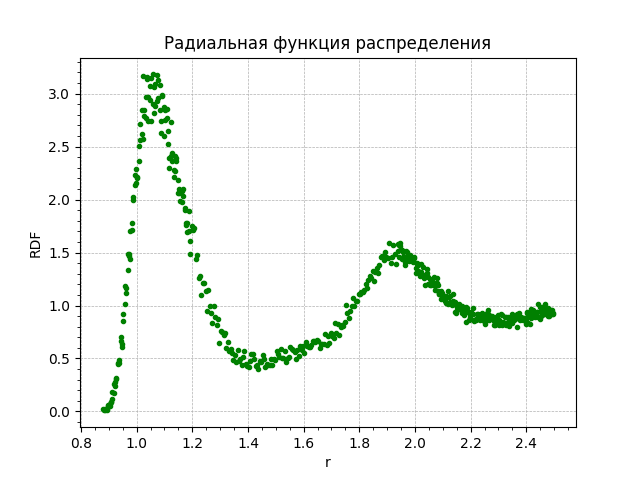
\includegraphics[width=\linewidth]{8.png}\\
        35000 шаг
    \end{center}
\end{minipage}

\section{Критерий Линдеманна}

Определим температуру плавления через критерий Линдеманна. Для этого построим зависимость среднеквадратичного отклонения частиц, нормированного на постоянную решетки, от температуры. Можно обнаружить начало фазового перехода. Принципиальное изменение зависимости среднеквадратичного смещения от температуры наблюдается при $T \approx 1.61$

\begin{center}
        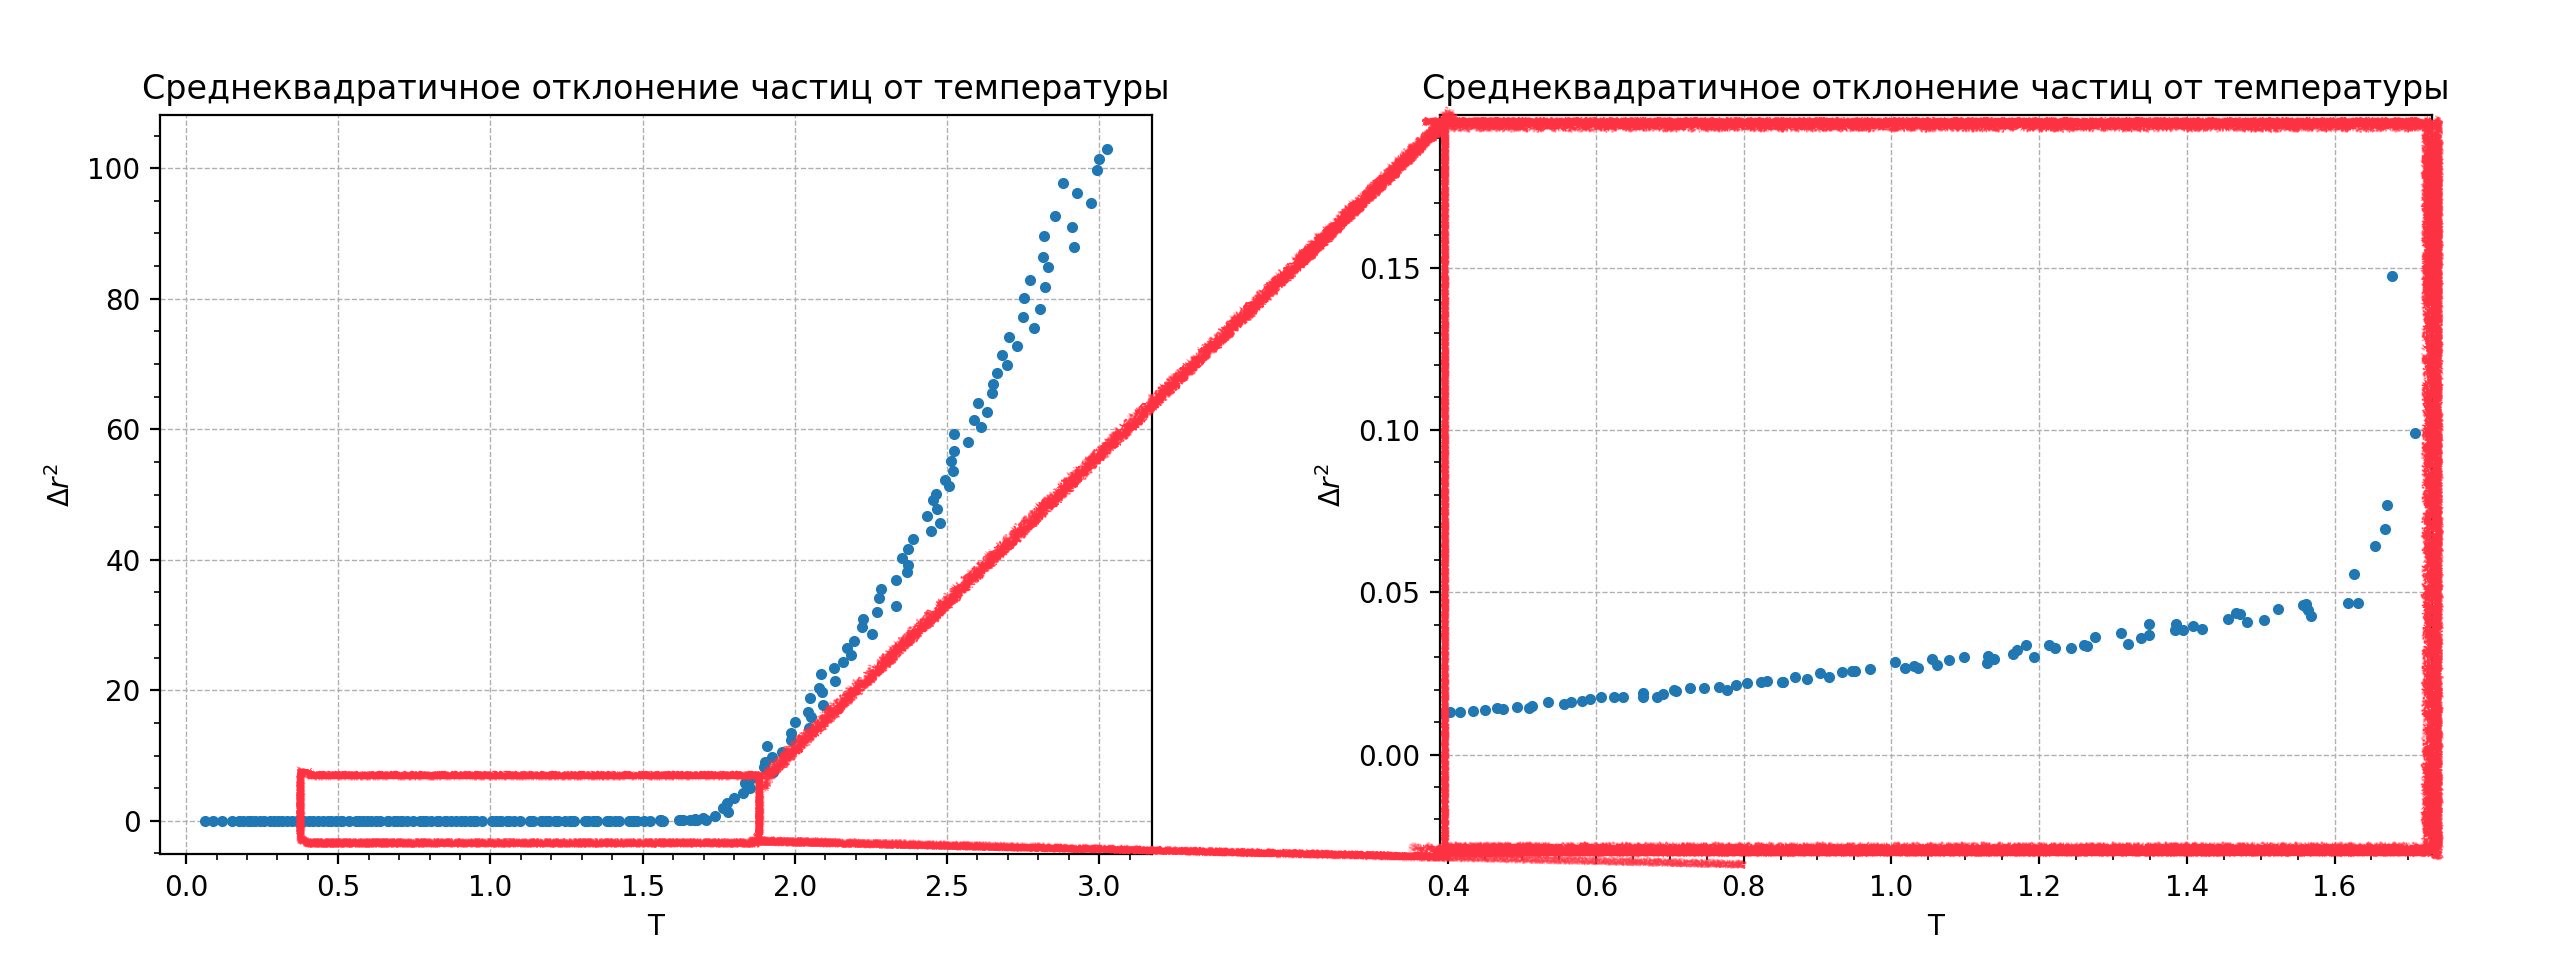
\includegraphics[width=\linewidth]{9.png}\\
        \end{center}


\section{Распределение отклонений частиц от положений равновесия}

Построим распределение отклонений частиц от положений равновесия для твердой фазы при постоянной температуре (T = 1.0). Можно заметить, что распределение похоже на Максвелловское, в чем можно убедиться, построив эту зависимость в линейных координатах. 

\begin{minipage}{0.47\textwidth}
    \begin{center}
        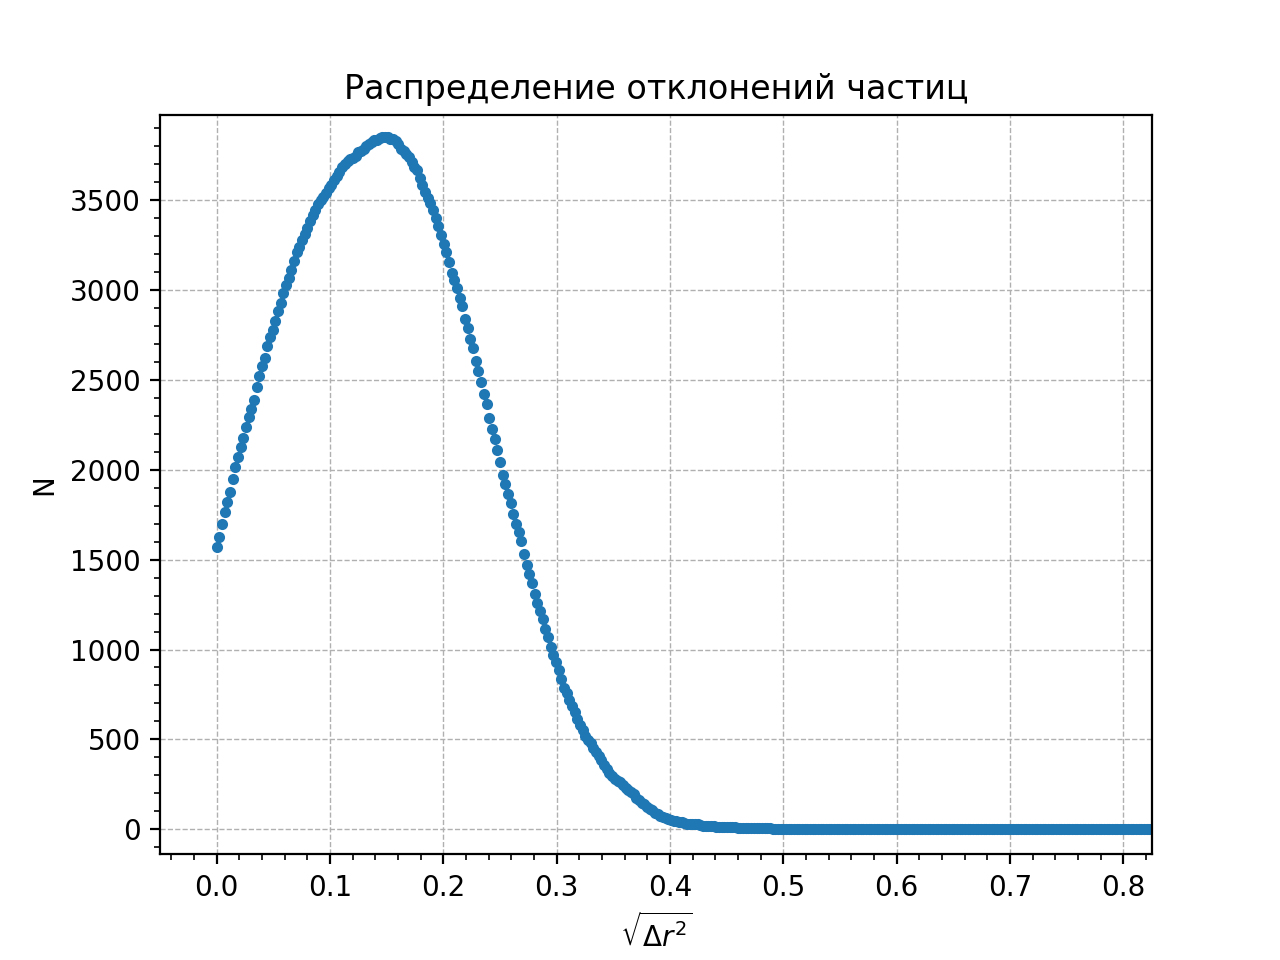
\includegraphics[width=0.9\linewidth]{name.png}\\
    \end{center}
   
\end{minipage}
\begin{minipage}{0.47\textwidth}
    \begin{center}
        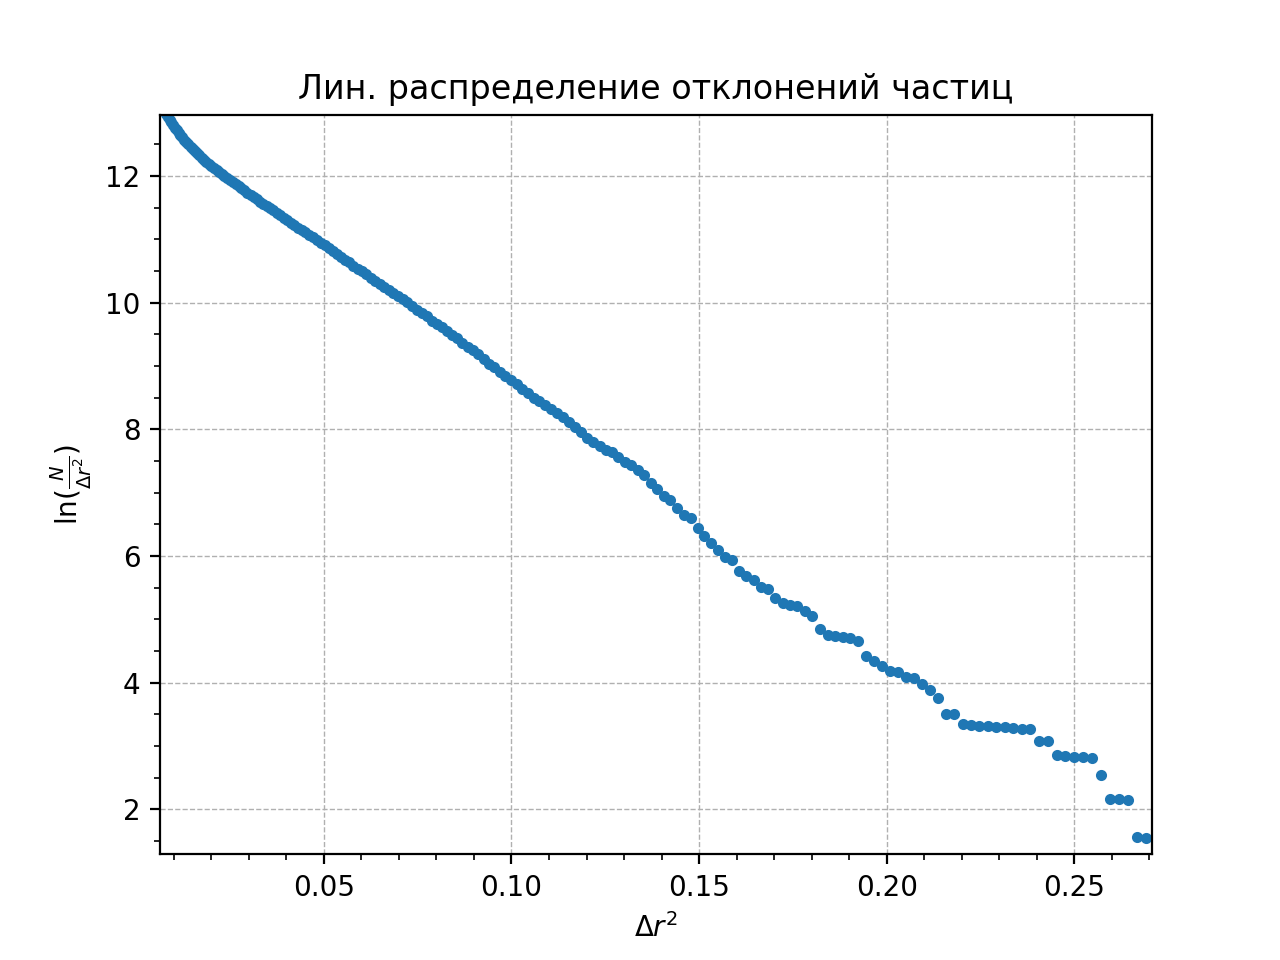
\includegraphics[width=0.9\linewidth]{nam.png}\\

    \end{center}
\end{minipage}


\section{Рассчет зависимости параметра негауссовости от температуры, определение температуры плавления}

\begin{minipage}{0.47\textwidth}
    Рассчитаем зависимость параметра негауссовости от температуры, по ней определим температуру плавления,\\ T = 1.689. 
    
   $$\alpha_{2}(t)=\frac{3\left\langle\Delta r^{4}\right\rangle}{5\left\langle\Delta r^{2}\right\rangle^{2}}-1$$
   
\end{minipage}
\begin{minipage}{0.47\textwidth}
    \begin{center}
        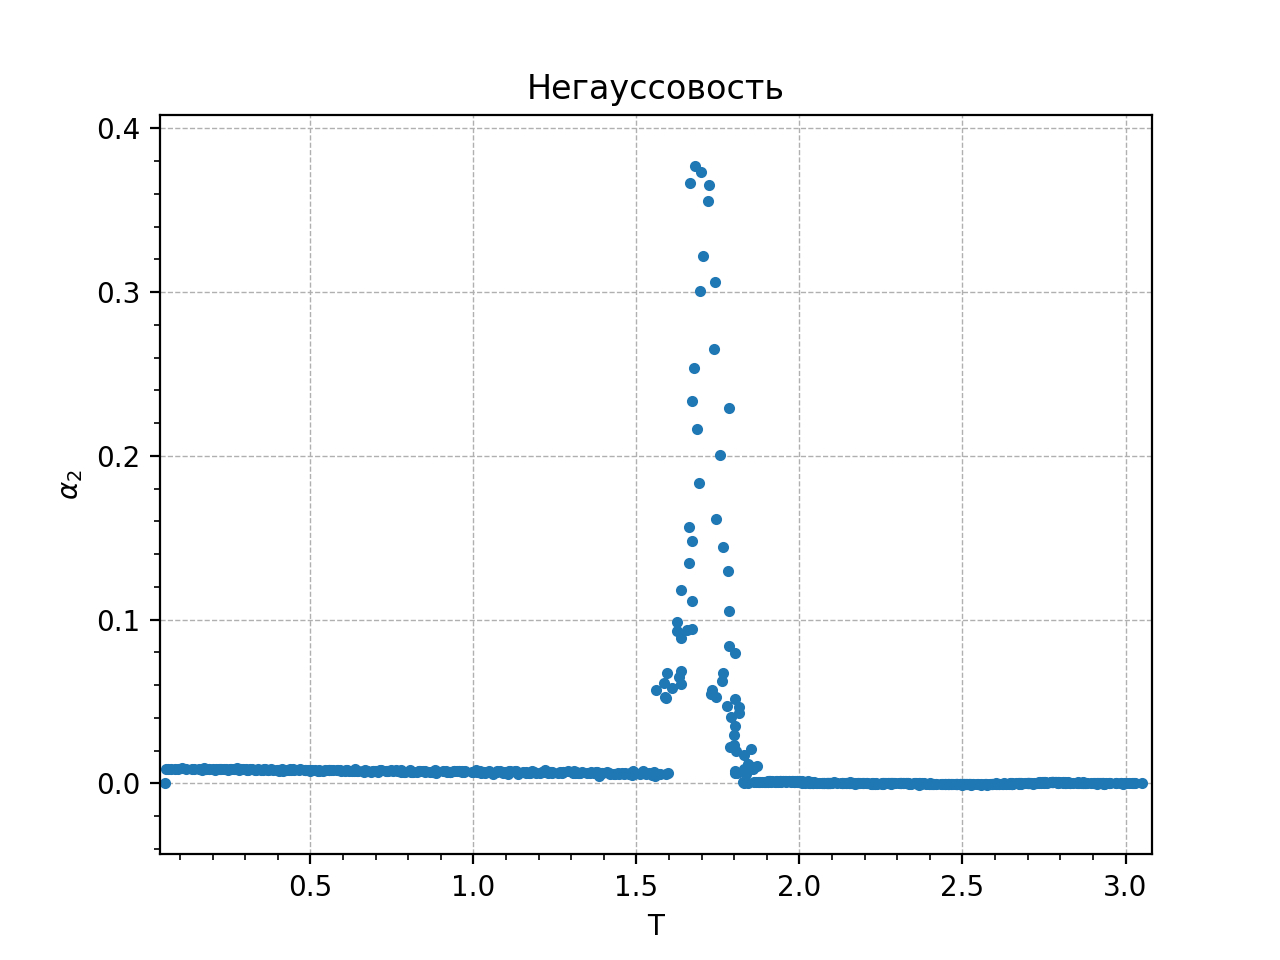
\includegraphics[width=\linewidth]{123.png}\\
    \end{center}
\end{minipage}


\section*{Вывод}\addcontentsline{toc}{section}{Вывод}

При выполнении работы можно было убедиться, что все методы дают немного различные результаты, но близкие друг к другу результаты, на основании которых можно сделать вывод о наличии фазового перехода. 

Подробнее код: \href{}{Github}

\end{document}
